\section{Αποτελέσματα}

\begin{frame}{Δείκτες}
	
	\setbeamertemplate{enumerate items}[square]

	\begin{enumerate}
		\item \textbf{Efficiency:} 
			\\[2mm]
			\begin{tabular}{c c c c} \toprule
				Επίπεδο & Συνολικά & Ένα \dvtrue & Δύο \dvtrue \\ \midrule
				$x-y$ & $0.95$ & $0.97$ & $0.91$ \\ 
				$\rho-z$ & $0.97$ & $0.99$ & $0.94$ \\ \bottomrule
			\end{tabular}
			\vspace{4mm}
		\item \textbf{Purity:} 
			\\[2mm]
			\begin{tabular}{c c c c} \toprule
				Επίπεδο & Συνολικά & Ένα \dvtrue & Δύο \dvtrue \\ \midrule
				$x-y$ & $0.71$ & $0.64$ & $0.90$ \\ 
				$\rho-z$ & $0.73$ & $0.65$ & $0.92$ \\ \bottomrule
			\end{tabular}	
	\end{enumerate}
\end{frame}

\beamerdefaultoverlayspecification{}

\begin{frame}{Δεδομένα από Ιστογράμματα}{Σφάλματα - Συνολικά}
	\centering
	\begin{tabular}{c c}
		\includegraphics[scale=0.38]{Errors-Total-3d} & 
		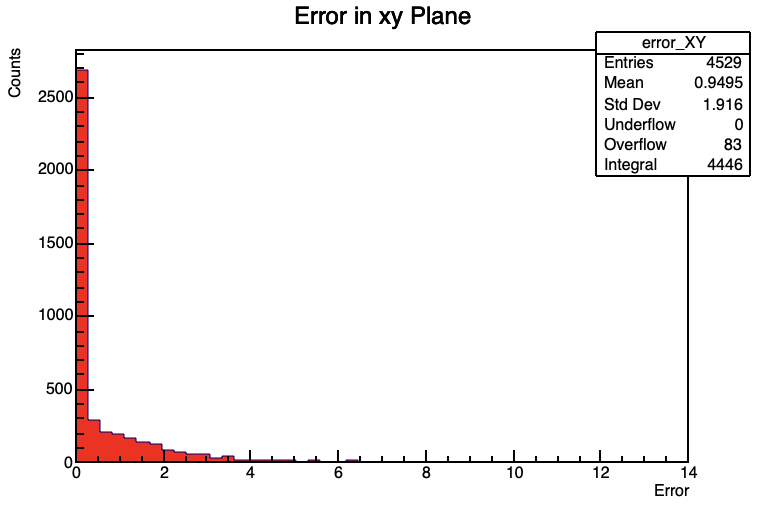
\includegraphics[scale=0.38]{Errors-Total-xy} \\[4mm]
		\small{Accuracy = $0.997$} & \small{Accuracy = $0.977$}
	\end{tabular}
\end{frame}

\begin{frame}{Δεδομένα από Ιστογράμματα}{Σφάλματα - Δεδομένα με Ένα \dvtrue}
	\centering
	\begin{tabular}{c c}
		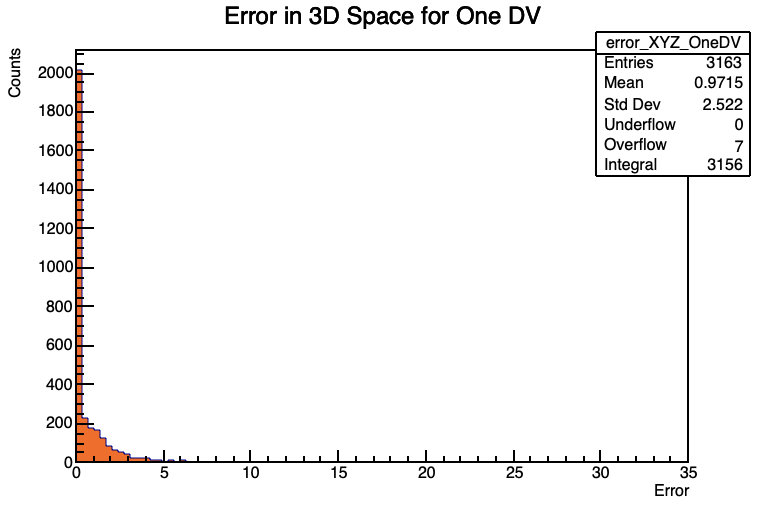
\includegraphics[scale=0.38]{Errors-OneDV-3D} & 
		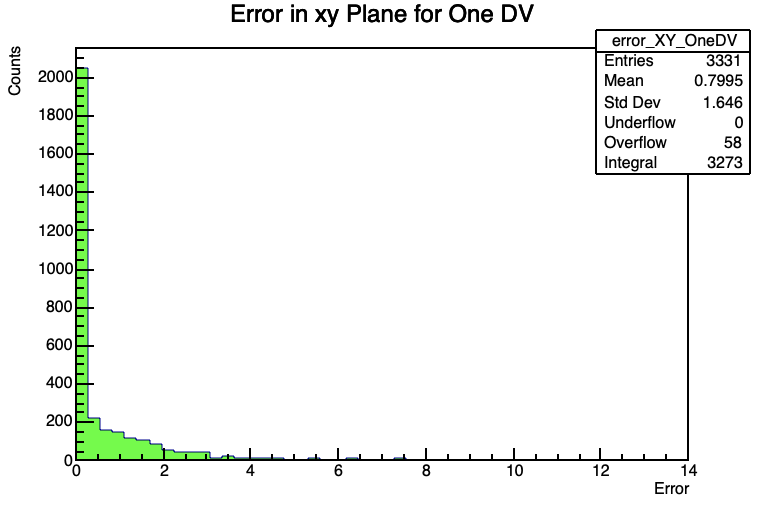
\includegraphics[scale=0.38]{Errors-OneDV-xy} \\[4mm]
		\small{Accuracy = $0.997$} & \small{Accuracy = $0.989$}
	\end{tabular}
\end{frame}

\begin{frame}{Δεδομένα από Ιστογράμματα}{Σφάλματα - Δεδομένα με Δύο \dvtrue}
	\centering
	\begin{tabular}{c c}
		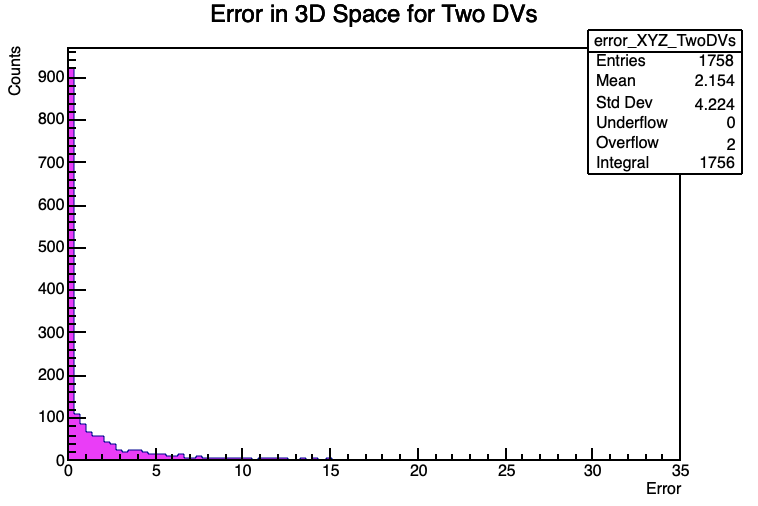
\includegraphics[scale=0.38]{Errors-TwoDVs-3D} & 
		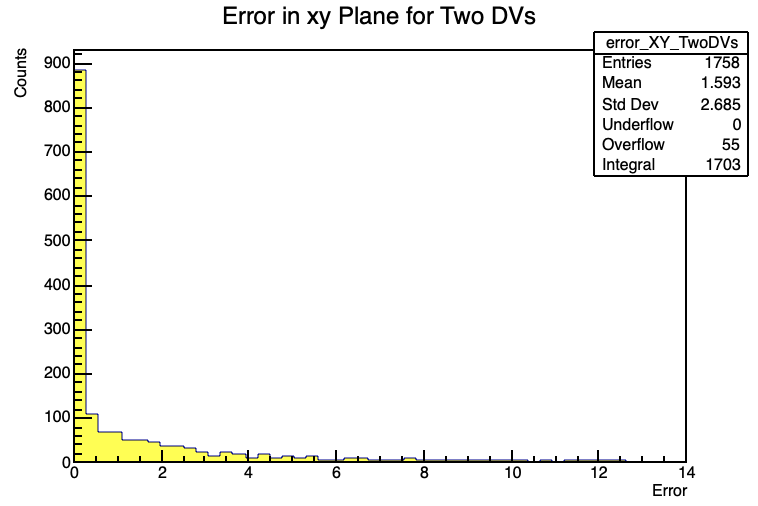
\includegraphics[scale=0.38]{Errors-TwoDVs-xy} \\[4mm]
		\small{Accuracy = $0.999$} & \small{Accuracy = $0.967$}
	\end{tabular}
\end{frame}

\begin{frame}{Δεδομένα από Ιστογράμματα}{Σχετικός Αριθμός \dvreco\ και \dvtrue}
	\centering
	\begin{tabular}{c c}
		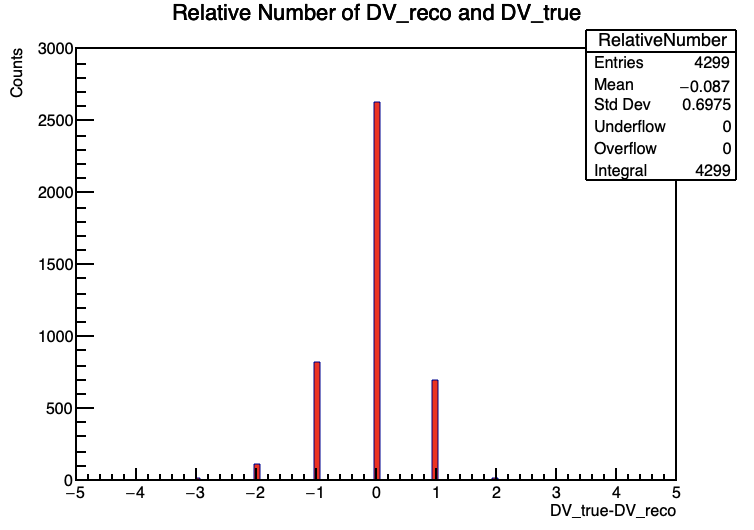
\includegraphics[scale=0.34]{Relative-Number-Total} &
		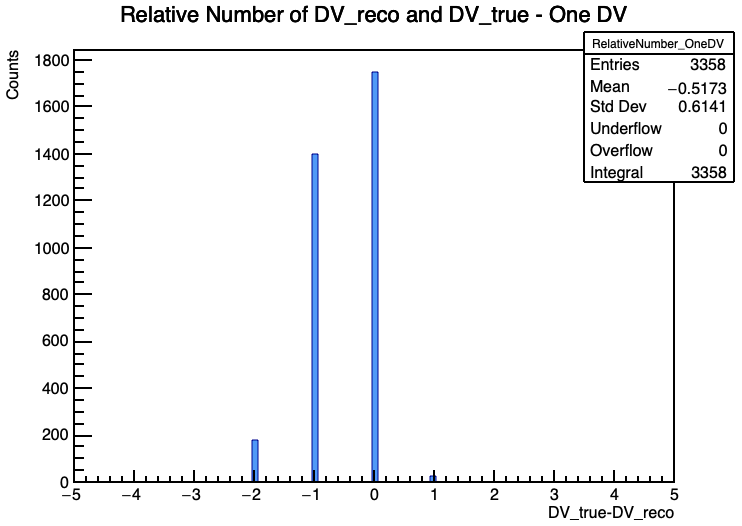
\includegraphics[scale=0.34]{Relative-Number-OneDV} 
	\end{tabular}
	\begin{tabular}{c}
		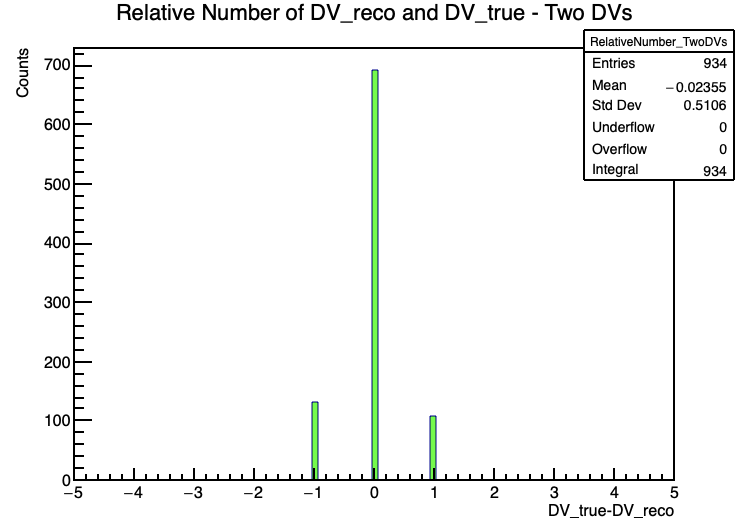
\includegraphics[scale=0.34]{Relative-Number-TwoDVs}
	\end{tabular}
\end{frame}

\begin{frame}{Δεδομένα από Ιστογράμματα}{Αριθμός \dvreco\ και \dvtrue\ - Συνολικά}
	\centering
	\begin{tabular}{c c}
		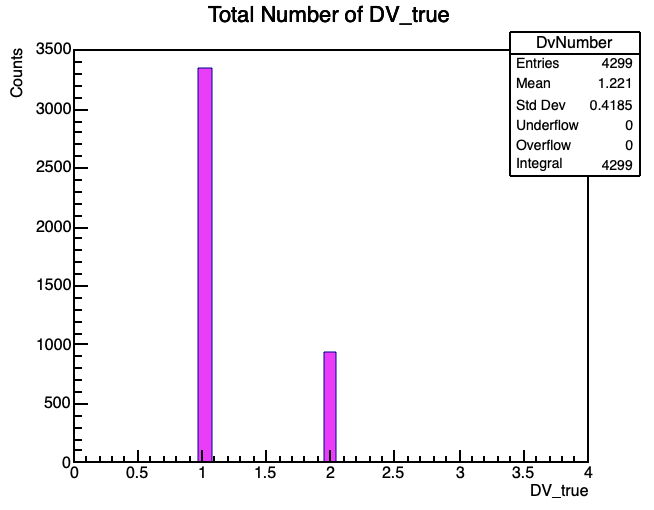
\includegraphics[scale=0.35]{DVtrue-Total} &
		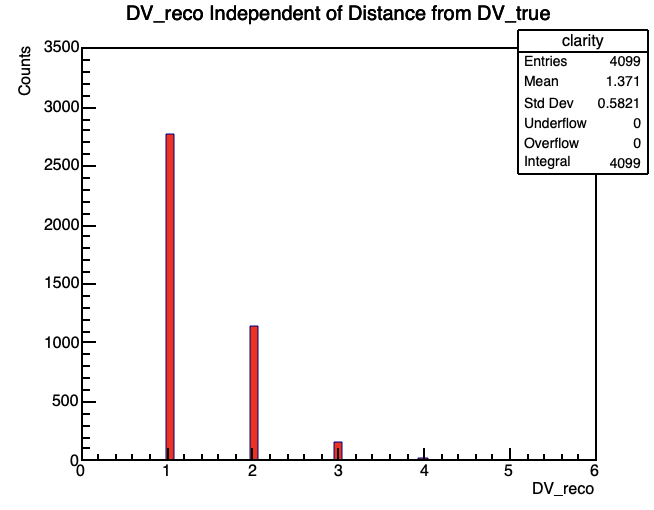
\includegraphics[scale=0.35]{DVreco-Total} \\
		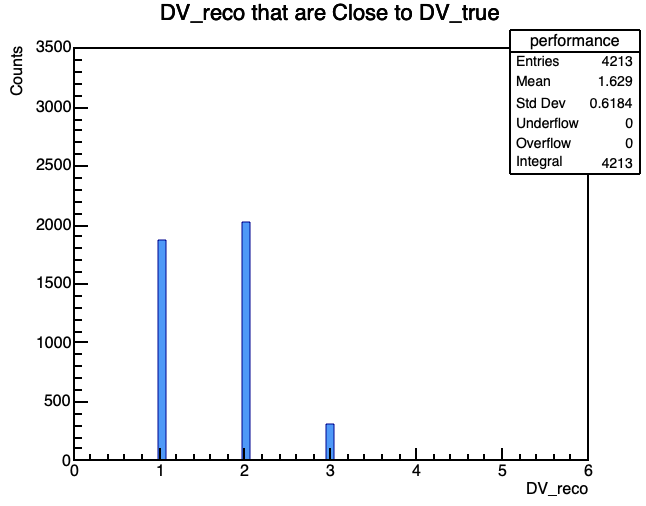
\includegraphics[scale=0.35]{DVreco-Close-Total} &
		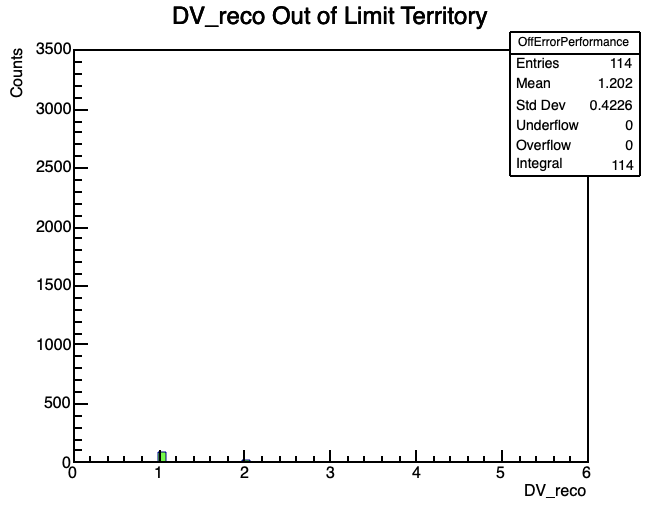
\includegraphics[scale=0.35]{DVreco-Far-Total}
	\end{tabular}
\end{frame}

\begin{frame}{Δεδομένα από Ιστογράμματα}{Αριθμός \dvreco\ και \dvtrue\ - Δεδομένα με Ένα \dvtrue}
	\centering
	\begin{tabular}{c c}
		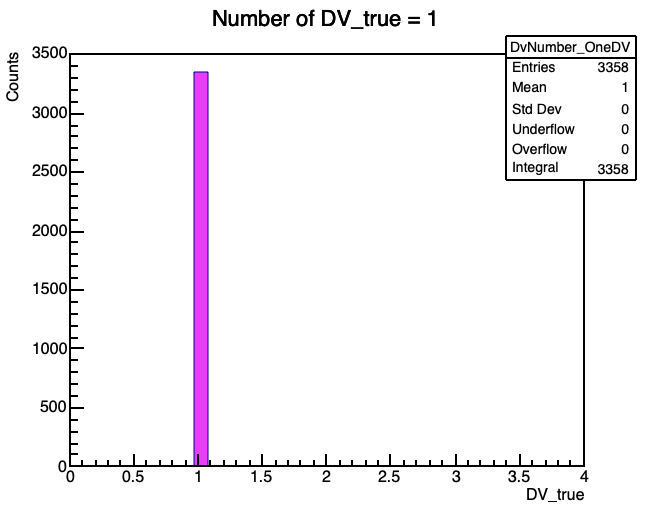
\includegraphics[scale=0.35]{DVtrue-OneDV} &
		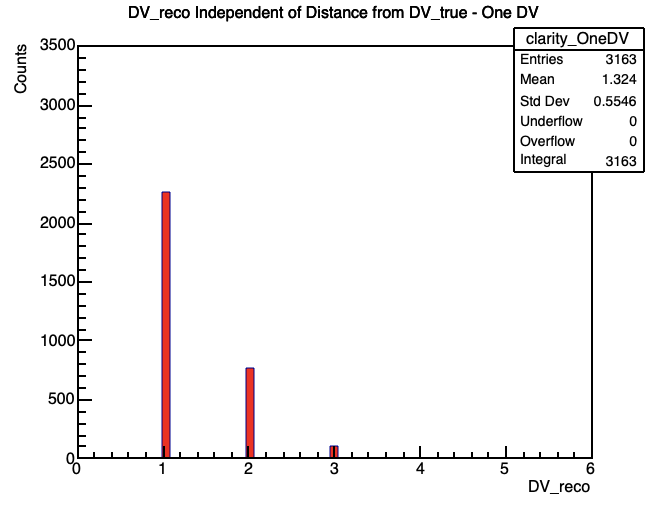
\includegraphics[scale=0.35]{DVreco-OneDV} \\
		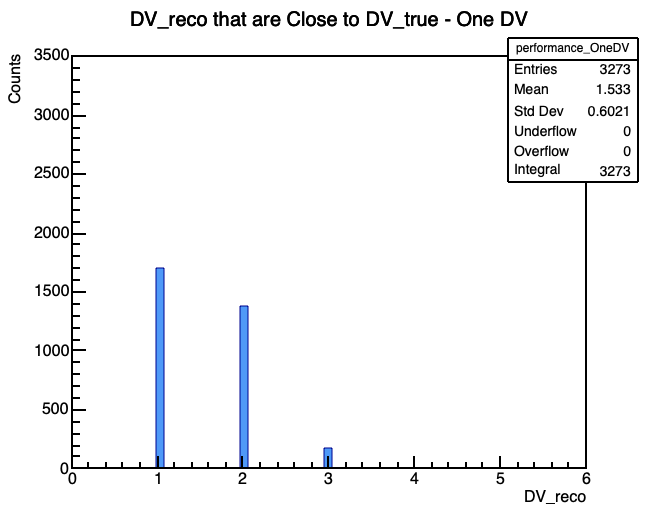
\includegraphics[scale=0.35]{DVreco-Close-OneDV} &
		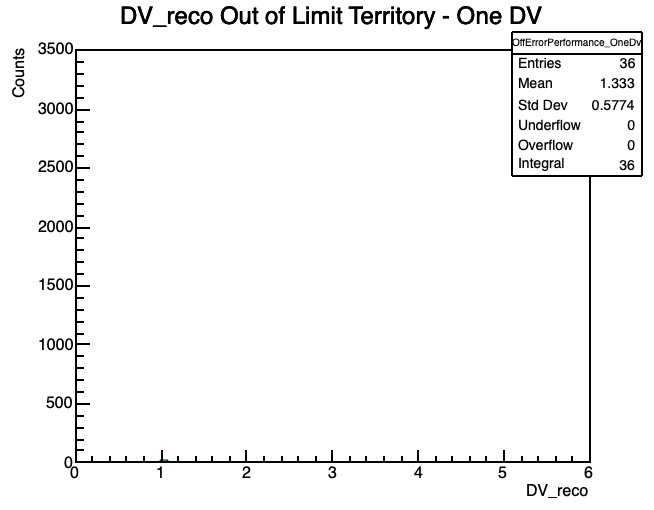
\includegraphics[scale=0.35]{DVreco-Far-OneDV}
	\end{tabular}
\end{frame}

\begin{frame}{Δεδομένα από Ιστογράμματα}{Αριθμός \dvreco\ και \dvtrue\ - Δεδομένα με Δύο \dvtrue}
	\centering
	\begin{tabular}{c c}
		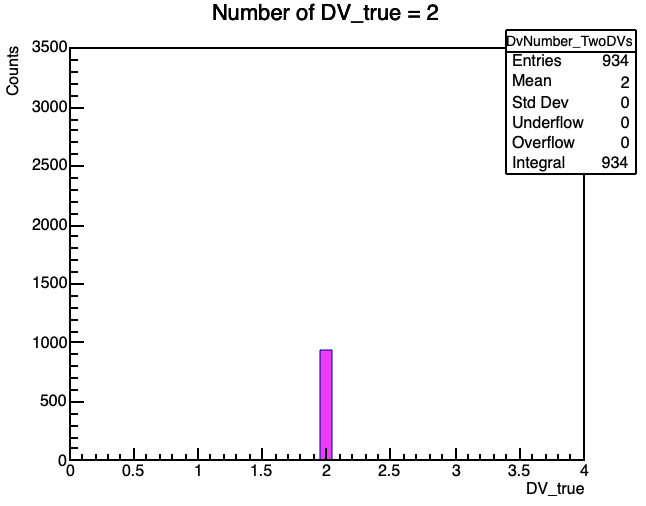
\includegraphics[scale=0.35]{DVtrue-TwoDVs} &
		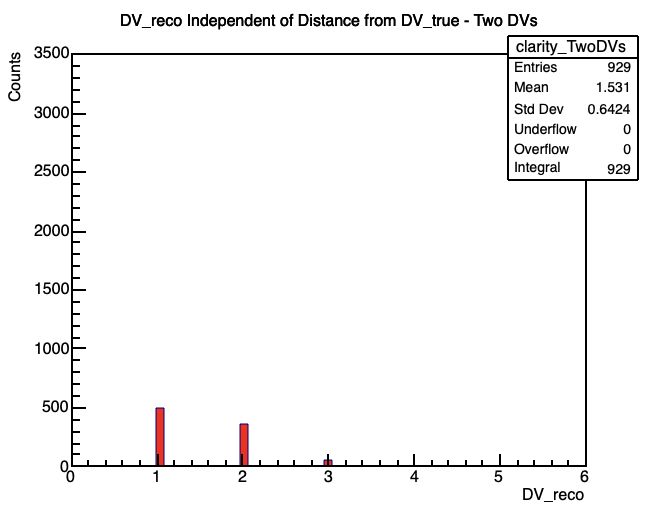
\includegraphics[scale=0.35]{DVreco-TwoDVs} \\
		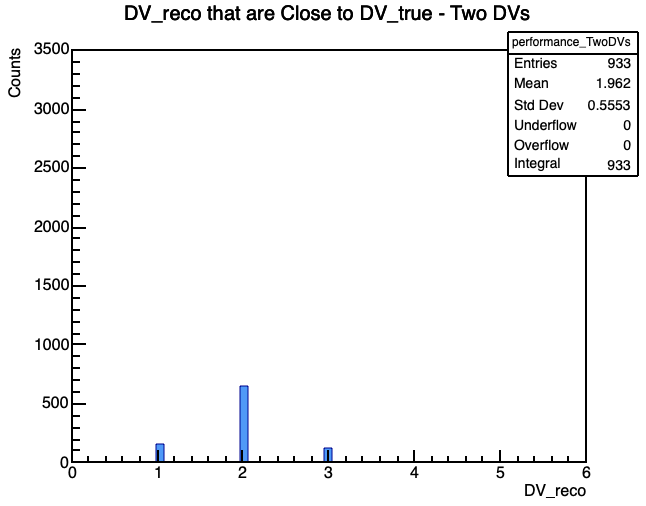
\includegraphics[scale=0.35]{DVreco-Close-TwoDVs} &
		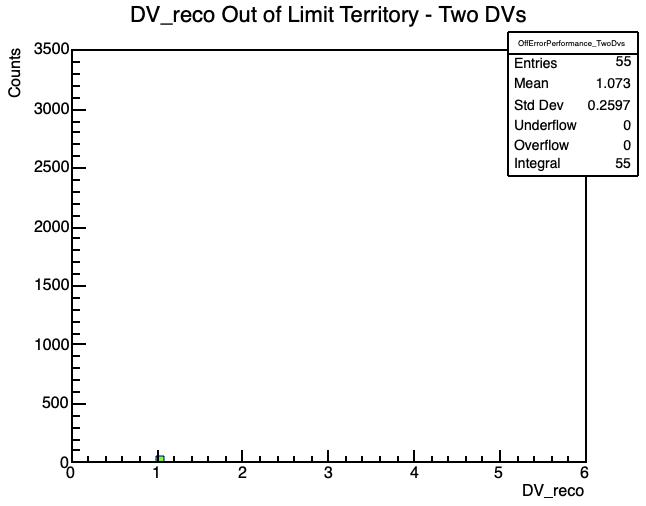
\includegraphics[scale=0.35]{DVreco-Far-TwoDVs}
	\end{tabular}
\end{frame}